\documentclass[main.tex]{subfiles}
\begin{document}

\subsection{Show that $\mathfrak{so}(2n)$ has a regular maximal subalgebra $\mathfrak{so}(2m)\times\mathfrak{so}(2n-2m)$. How does the spinor rep. of $\mathfrak{so}(2n)$ transform under the subalgebra?}
$\mathfrak{so}(2n)=D_n$ 
\begin{center}
  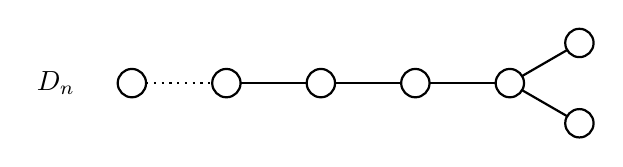
\begin{tikzpicture}[scale=.6]
    \draw (-1,0) node[anchor=east]  {$D_n$};
    \foreach \x in {0,...,4}
    \draw[xshift=\x cm,thick] (\x cm,0) circle (.3cm);
    \draw[xshift=8 cm,thick] (30: 17 mm) circle (.3cm);
    \draw[xshift=8 cm,thick] (-30: 17 mm) circle (.3cm);
    \draw[dotted,thick] (0.3 cm,0) -- +(1.4 cm,0);
    \foreach \y in {1.15,...,3.15}
    \draw[xshift=\y cm,thick] (\y cm,0) -- +(1.4 cm,0);
    \draw[xshift=8 cm,thick] (30: 3 mm) -- (30: 14 mm);
    \draw[xshift=8 cm,thick] (-30: 3 mm) -- (-30: 14 mm);
  \end{tikzpicture}
\end{center}

$D_n'$ is 
\begin{figure}[H] 
\centering
  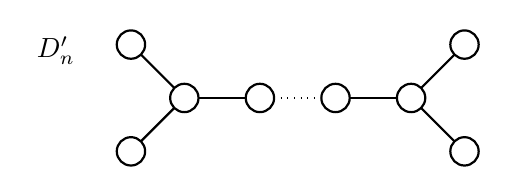
\begin{tikzpicture}[scale=.6]
    \draw (-3.71,1) node[anchor=east]  {$D_n'$};
    \draw[thick] (-1.81, 0.21 ) -- +(-0.707 ,0.707);
    \draw[thick] (-2.73,1.13) circle (.3);
    \draw[thick] (-1.81, -0.21 ) -- +(-0.707 ,-0.707);
    \draw[thick] (-2.73,-1.13) circle (.3);
    \draw[thick] (-1.6,0) circle (.3);
    \draw[thick] (-0.3, 0 ) -- +(-1 ,0);
    \draw[thick] (0,0) circle (.3);
    \draw[dotted] (0.3, 0 ) -- +(1 ,0);
    \draw[thick] (1.6,0) circle (.3);
    \draw[thick] (1.9, 0 ) -- +(1 ,0);
    \draw[thick] (3.2,0) circle (.3);
    \draw[thick] (3.41, 0.21 ) -- +(0.707 ,0.707);
    \draw[thick] (4.33,1.13) circle (.3);
    \draw[thick] (3.41, -0.21 ) -- +(0.707 ,-0.707);
    \draw[thick] (4.33,-1.13) circle (.3);
  \end{tikzpicture}
\end{figure}

removing the $m^{\text{th}}$ circle from $D_n'$ gives 
\begin{figure}[H] 
\centering
  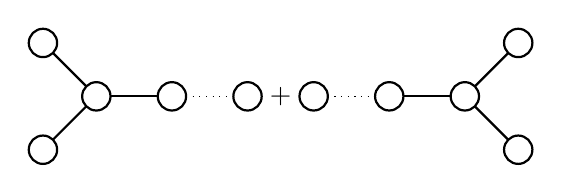
\begin{tikzpicture}[scale=.6]
    \draw[thick] (-1.81, 0.21 ) -- +(-0.707 ,0.707);
    \draw[thick] (-2.73,1.13) circle (.3);
    \draw[thick] (-1.81, -0.21 ) -- +(-0.707 ,-0.707);
    \draw[thick] (-2.73,-1.13) circle (.3);
    \draw[thick] (-1.6,0) circle (.3);
    \draw[thick] (-0.3, 0 ) -- +(-1 ,0);
    \draw[thick] (0,0) circle (.3);
    \draw[dotted] (0.3, 0 ) -- +(1 ,0);
    \draw[thick] (1.6,0) circle (.3);
    
    \node at (2.3,0) {$+$};
    
    \draw[thick] (3.0,0) circle (.3);
    \draw[dotted] (3.3, 0 ) -- +(1 ,0);
    \draw[thick] (4.6,0) circle (.3);
    \draw[thick] (4.9, 0 ) -- +(1 ,0);
    \draw[thick] (6.2,0) circle (.3);
    \draw[thick] (6.41, 0.21 ) -- +(0.707 ,0.707);
    \draw[thick] (7.33,1.13) circle (.3);
    \draw[thick] (6.41, -0.21 ) -- +(0.707 ,-0.707);
    \draw[thick] (7.33,-1.13) circle (.3);
  \end{tikzpicture}
\end{figure}
which is $D_{n-m}+D_{m}=\mathfrak{so}(2n-2m)+\mathfrak{so}(2m)$.

The $\mathfrak{so}(2n)$ spinor transforms on first $m$ components as a $\mathfrak{so}(2m)$ spinor and on the other $m+1...n-m$ components as a $\mathfrak{so}(2n-2m)$ spinor. 

\subsection{Show that $\mathfrak{so}(2n+1)$ has a regular maximal subalgebra $\mathfrak{so}(2m)\times\mathfrak{so}(2n-2m+1)$. How does the spinor rep. of $\mathfrak{so}(2n+1)$ transform under the subalgebra?}

$\mathfrak{so}(2n+1)=B_n$ 
\begin{center}
  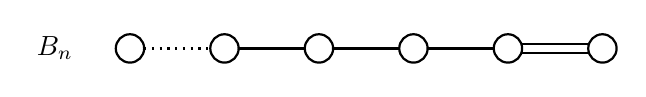
\begin{tikzpicture}[scale=.6]
    \draw (-1,0) node[anchor=east]  {$B_n$};
    \foreach \x in {0,...,4}
    \draw[xshift=\x cm,thick] (\x cm,0) circle (.3cm);
    \draw[xshift=5 cm,thick,] (5 cm, 0) circle (.3 cm);
    \draw[dotted,thick] (0.3 cm,0) -- +(1.4 cm,0);
    \foreach \y in {1.15,...,3.15}
    \draw[xshift=\y cm,thick] (\y cm,0) -- +(1.4 cm,0);
    \draw[thick] (8.3 cm, .1 cm) -- +(1.4 cm,0);
    \draw[thick] (8.3 cm, -.1 cm) -- +(1.4 cm,0);
  \end{tikzpicture}
\end{center}
So that $B_n'$ is
\begin{figure}[H] 
\centering
  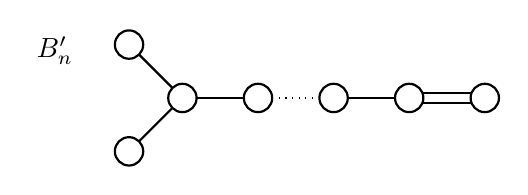
\begin{tikzpicture}[scale=.6]
    \draw (-3.71,1) node[anchor=east]  {$B_n'$};
    \draw[thick] (-1.81, 0.21 ) -- +(-0.707 ,0.707);
    \draw[thick] (-2.73,1.13) circle (.3);
    \draw[thick] (-1.81, -0.21 ) -- +(-0.707 ,-0.707);
    \draw[thick] (-2.73,-1.13) circle (.3);
    \draw[thick] (-1.6,0) circle (.3);
    \draw[thick] (-0.3, 0 ) -- +(-1 ,0);
    \draw[thick] (0,0) circle (.3);
    \draw[dotted] (0.3, 0 ) -- +(1 ,0);
    \draw[thick] (1.6,0) circle (.3);
    \draw[thick] (1.9, 0 ) -- +(1 ,0);
    \draw[thick] (3.2,0) circle (.3);
    \draw[thick] (4.8,0) circle (.3);
    \draw[thick] (3.5, 0.1 ) -- +(1 ,0);
    \draw[thick] (3.5, -0.1 ) -- +(1 ,0);
  \end{tikzpicture}
\end{figure}
Removing the $m^{\text{th}}$ circle from $B_n'$ gives
  
\begin{figure}[H] 
\centering
  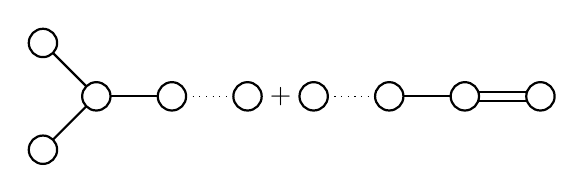
\begin{tikzpicture}[scale=.6]
    \draw[thick] (-1.81, 0.21 ) -- +(-0.707 ,0.707);
    \draw[thick] (-2.73,1.13) circle (.3);
    \draw[thick] (-1.81, -0.21 ) -- +(-0.707 ,-0.707);
    \draw[thick] (-2.73,-1.13) circle (.3);
    \draw[thick] (-1.6,0) circle (.3);
    \draw[thick] (-0.3, 0 ) -- +(-1 ,0);
    \draw[thick] (0,0) circle (.3);
    \draw[dotted] (0.3, 0 ) -- +(1 ,0);
    \draw[thick] (1.6,0) circle (.3);
    \node at (2.3,0) {$+$};
    \draw[thick] (3.0,0) circle (.3);
    \draw[dotted] (3.3, 0 ) -- +(1 ,0);
    \draw[thick] (4.6,0) circle (.3);
    \draw[thick] (4.9, 0 ) -- +(1 ,0);
    \draw[thick] (6.5, -0.1 ) -- +(1 ,0);
    \draw[thick] (6.5, 0.1 ) -- +(1 ,0);
    \draw[thick] (6.2,0) circle (.3);
    \draw[thick] (7.8,0) circle (.3);
  \end{tikzpicture}
\end{figure}
which is $D_m+B_{n-m}=\mathfrak{so}(2m)+\mathfrak{so}(2n-2m+1)$.

The spinor rep. of $\mathfrak{so}(2n+1)$ transforms under the subalgebra as a $\mathfrak{so}(2m)$ component spinor on the first $m$ components and as a $\mathfrak{so}(2n-2m+1)$ spinor on the remaining $m+1...n-m$ components.

\subsection{Show that $\mathfrak{so}(4)$ has the same algebra as $\mathfrak{su}(2)\times\mathfrak{su}(2)$ and thus is not simple, however the spinor arguments still apply, explain how.}

To show we can show that $\mathfrak{so}(4)\cong\mathfrak{su}(2)\times\mathfrak{su}(2)$ by verifying that the two algebras have the same commutation relations and that there exists a one-to-one mapping between the generators of the two algebras. 

$\mathfrak{so}(4)$ has $\frac{n(n-1)}{2}=\frac{4\cdot3}{2}=6$ generators and is of rank $2$ with three hermitian generators
\begin{align}
h_3=&M_{56}=-\frac{1}{2}\sigma_3\otimes\sigma_3\equiv T_{23}\\
h_1=&M_{16}=-\frac{1}{2}\sigma_3\otimes\sigma_1\equiv T_{21}\\
h_2=&M_{26}=-\frac{1}{2}\sigma_3\otimes\sigma_2\equiv T_{22}.
\end{align}

The other 3 generators are given by commutation 
\begin{align}
[h1,h3]&=\frac{\img}{2}\mathbb{I}\otimes\sigma_2\equiv T_{12}\\
[h2,h3]&=\frac{\img}{2}\mathbb{I}\otimes\sigma_1\equiv T_{11}\\
[h1,h2]&=\frac{\img}{2}\mathbb{I}\otimes\sigma_3\equiv T_{13}.
\end{align}
 Then, constructing the commutators
\begin{align}
[T_{1a},T_{1b}]&=2\img\epsilon_{abc}T_{1c}\\
[T_{2a},T_{2b}]&=2\img\epsilon_{abc}T_{1c}\\
[T_{1a},T_{2b}]&=2\img\epsilon_{abc}T_{2c}.
\end{align}
We know from Problem(\ref{Sec:8B}) which describes the algebra $\mathfrak{su}(2)\times\mathfrak{su}(2)$ has the commutation relations
\begin{align}
[\sigma_a\otimes\mathbb{I},\sigma_b\otimes\mathbb{I}]&=2\img\epsilon_{abc}\sigma_c\otimes\mathbb{I}\\
[\sigma_a\otimes\eta_1,\sigma_b\otimes\eta_1]&=2\img\epsilon_{abc}\sigma_c\otimes\mathbb{I}\\
[\sigma_a\otimes\mathbb{I},\sigma_b\otimes\eta_1]&=2\img\epsilon_{abc}\sigma_c\otimes\eta_1.
\end{align}
Thus we can see that an appropriate one-to-one mapping is
\begin{align}
T_{1a}&\rightarrow\sigma_a\otimes\mathbb{I}\\
T_{2a}&\rightarrow\sigma_a\otimes\eta_1
\end{align} and therefore, $\mathfrak{so}(4)\cong\mathfrak{su}(2)\times\mathfrak{su}(2)$.
The two simple roots in $\mathfrak{so}(4)$ are $\alpha^1=(e^1-e^2)$ and $\alpha^2=(e^1+e^2)$ so $\alpha^1\cdot\alpha^2=0$ just as, for arbitrary $n$ in $\mathfrak{so}(2n)$, $\alpha^n\cdot\alpha^{n+1}=0$ and the two simple roots in $\mathfrak{so}(4)$ are connected in the same way as the roots $\alpha^n$, $\alpha^{n+1}=0$ in $\mathfrak{so}(2n)$.

\subsection{Show that the $\mathfrak{so}(6)$ algebra and the $\mathfrak{su}(4)$ algebra are equivalent with the $4$ of $\mathfrak{su}(4)$ correspondig to a spinor rep of $\mathfrak{so}(6)$. In $\mathfrak{su}(4)$, $4\otimes4=6\oplus10$. The $6$ is the vector rep. of $\mathfrak{so}(6)$, what is the $10$?}
Both $\mathfrak{so}(6)$ and $\mathfrak{su}(4)$ have $15$ generators. 

The 15 generators of $\mathfrak{su}(4)$ may be constructed by the $15$ independent, traceless, hermitian matrices $T_{ab}=\sigma_a\otimes\sigma_b$, $T_{0a}=\mathbb{I}\otimes\sigma_a$ and $T_{a0}=\sigma_a\otimes\mathbb{I}$ which form a basis for the $\mathfrak{su}(4)$ Lie algebra with commutators
\begin{align}
[T_{ab},T_{mn}]&=\sigma_a\sigma_m\otimes\sigma_b\sigma_n-\sigma_m\sigma_a\otimes\sigma_n\sigma_b\\
&=(\img\epsilon_{ami}\sigma_i+\delta_{am}\mathbb{I})\otimes(\img\epsilon_{bnj}\sigma_j+\delta_{bn}\mathbb{I})-(\img\epsilon_{mai}\sigma_i+\delta_{ma}\mathbb{I})\otimes(\img\epsilon_{nbj}\sigma_j+\delta_{nb}\mathbb{I})\\
&=2\img\epsilon_{ami}\delta_{bn}\sigma_i\otimes\mathbb{I}+2\img\epsilon_{bnj}\delta_{am}\mathbb{I}\otimes\sigma_j\\
&=2\img\epsilon_{ami}\delta_{bn}T_{i0}+2\img\epsilon_{bnj}\delta_{am}T_{0j}\\
[T_{ab},T_{0m}]&=2\img\epsilon_{bmj}T_{aj}\\
[T_{ab},T_{m0}]&=2\img\epsilon_{amj}T_{jb}\\
[T_{0a},T_{m0}]&=0.
\end{align}

The $\mathfrak{so}(6)$ generators may be obtained from the following four Hermitian matrices
\begin{align}
M_{56}&=\frac{1}{2}\sigma_3\otimes\sigma_3\equiv X_{33}\\
M_{16}&=\frac{1}{2}\sigma_1\otimes\mathbb{I}\equiv X_{10}\\
M_{36}&=\frac{1}{2}\sigma_3\otimes\sigma_1\equiv X_{31}\\
M_{46}&=\frac{1}{2}\sigma_3\otimes\sigma_2\equiv X_{32}.
\end{align}

The other generators can be constructed via commutation
\begin{align}
[X_{3i},X_{3j}]&=\frac{1}{2}\mathbb{I}\otimes\img\epsilon_{ijk}\sigma_{k}\equiv X_{0k}\\
[X_{3i},X_{10}]&=\frac{1}{2}\sigma_2\otimes\img\sigma_{i}\equiv X_{2i}\\
[X_{3i},[X_{3j},X_{10}]]&=[X_{3i},X_{2j}]=\frac{1}{2}\sigma_1\otimes\img\epsilon_{ijk}\sigma_{k}\equiv X_{1k}\\
[X_{3i},X_{0i}]&=\frac{1}{2}\sigma_3\otimes\mathbb{I}\equiv X_{30}\\
[X_{3i},X_{3j}]&=\frac{1}{2}\sigma_2\otimes\mathbb{I}\equiv X_{20}
\end{align}

So the algebra closes. All together,
\begin{align}
X_{ij}&=\frac{1}{2}\sigma_i\otimes\sigma_j\\
X_{j0}&=\frac{1}{2}\sigma_j\otimes\mathbb{I}\\
X_{0j}&=\frac{1}{2}\mathbb{I}\otimes\sigma_j.
\end{align}

Thus $\mathfrak{so}(6)\cong\mathfrak{su}(4)$ with the one-to-one mapping $X_{\mu\nu}\rightarrow\frac{1}{2}T_{\mu\nu}$, $\mu,\nu=0...4$, $\mu+\nu\neq0$.
\end{document}